\chapter{Design}
\label{Design}

In this chapter, we are going to describe the design part of the solution.

\section{Main components}

First of all, let us briefly have a look at the main components:

\begin{figure}[!htb]
    \setlength{\fboxsep}{4pt}%
    \setlength{\fboxrule}{1pt}%
    \fbox{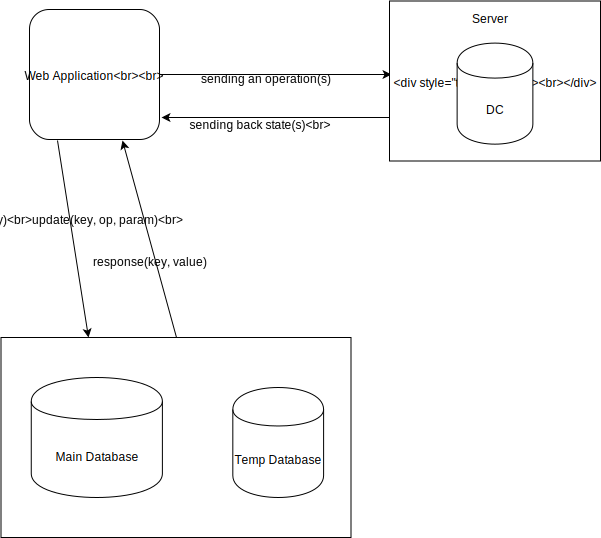
\includegraphics[width=\linewidth]{images/pseudocode/diagram.png}}
    \caption{An overview of the system's design.}
    \label{fig:design1}
  \end{figure}

\subsection*{Web Application}

It is a client application, which runs in the web-browser and supports interactive commands performed by user. It sits on top of the database layer.

\vspace{5mm}These are the supported commands:

\begin{itemize}
    \item \textit{read(key)} -- an asynchronous function that pulls database changes concerning the key that the user passed.
    \item \textit{update(key, op)}  -- an asynchronous function that processes user-made update.
     \begin{itemize}
         \item \textit{key}: a key, which is going to be updated;
         \item \textit{op}: an operation, which is going to be performed on the key;
     \end{itemize}
  \end{itemize}

\subsection*{Server}

It is a configured AntidoteDB server that supports the following scenarios:

\begin{itemize}
    \item receiving an array of operations performed on a CRDT-object according to the key and applying them on the server;
    \item sending back to the client the state of requested CRDT-object / objects according to their state on the server;
    %\item sending back states of all stored CRDT-objects, if a specific object was not asked for; 
\end{itemize}

\subsection*{A database layer}

This layer should consist of two databases - \textit{main database} and a \textit{temporary} one.

\begin{itemize}
	\item Main database: this database stores the actual states of CRDT-objects.
	\item Temporary database: this database stores user-added operations performed on the states, which are stored in the main database.
\end{itemize}

When a user performs \textit{read} by \textit{key} operation from cache, the following actions are taking place:

\begin{itemize}
\item Firstly, the state of the object \textit{\textbf{O}} is going to be found by \textit{\textbf{key}} in the \textit{Main database}
\item Next, from the \textit{temporary database}, operations \textit{\textbf{o}} performed on the object \textit{\textbf{O}} are selected
\item Afterwards, selected operations \textit{\textbf{o}} applied on the object \textit{\textbf{O}}.
\item Finally, the object from the previous step is returned back as a response to the application.
\end{itemize} 

\begin{codelisting}[!h]  
    \caption[A prototype for the start function.]{The example behaviour for the function, which should run at the start of the application.}
    \lstinputlisting[language=JavaScript]{jslistings/start_offline.js}
    \label{codelst:lst1}
\end{codelisting}

Above you can look at the function, which should run at the starting point of the application. 

\begin{codelisting}[!h]   
    \caption[A prototype for the read function.]{The example behaviour for the function, which should run at the read time.}
    \lstinputlisting[language=JavaScript]{jslistings/read_offline.js}
    \label{codelst:lst2}
\end{codelisting}
\begin{codelisting}[!h]   
    \caption[A prototype for the update function.]{The example behaviour for the function, which should run at the update time.}
    \lstinputlisting[language=JavaScript]{jslistings/update_offline.js}
    \label{codelst:lst3}
\end{codelisting}